\chapter{Конструкторский раздел}
В данном разделе представлены требования к разрабатываемому ПО и схемы алгоритмов умножения матриц.

\section{Требования к ПО}

К программе предъявляется ряд требований:
\begin{itemize}
	\item корректное умножение матриц размером до $[N \times N]$, где $N\in[0:2000]$;
	\item при матрицах неправильных размеров программа не должна аварийно завершаться.
\end{itemize}

\section{Схемы алгоритмов}
Ниже представлены схемы следующих алгоритмов сортировки:
\begin{itemize}
	\item схема классического алгоритма умножения матриц (Рисунок \ref{img:m_std});
	\item схема алгоритма Винограда (рисунки \ref{img:m_winograd} - \ref{img:m_winograd2});
\end{itemize}


\begin{figure}
	\center{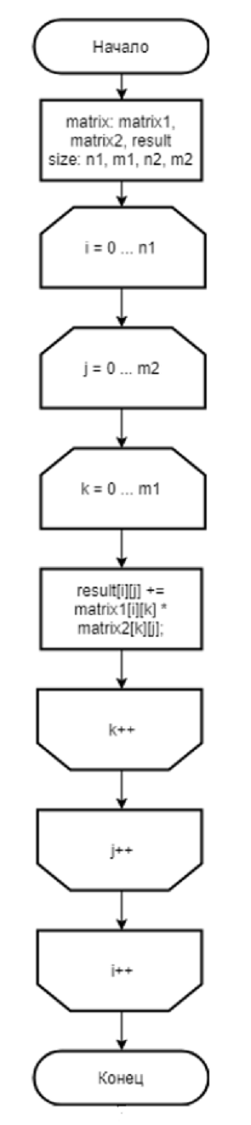
\includegraphics[width=0.3\linewidth]{inc/img/m_std}}
	\caption{Схема классического алгоритма умножения матриц}
\end{figure}

\begin{figure}
	\center{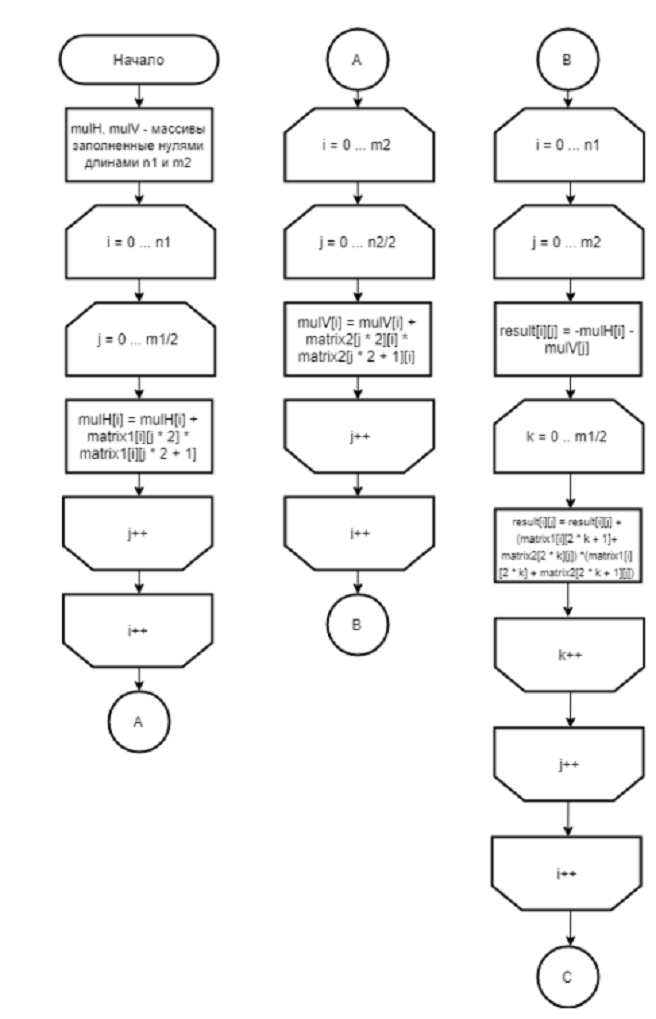
\includegraphics[width=1\linewidth]{inc/img/m_winograd}}
	\caption{Схема алгоритма Винограда}
\end{figure}

\begin{figure}
	\center{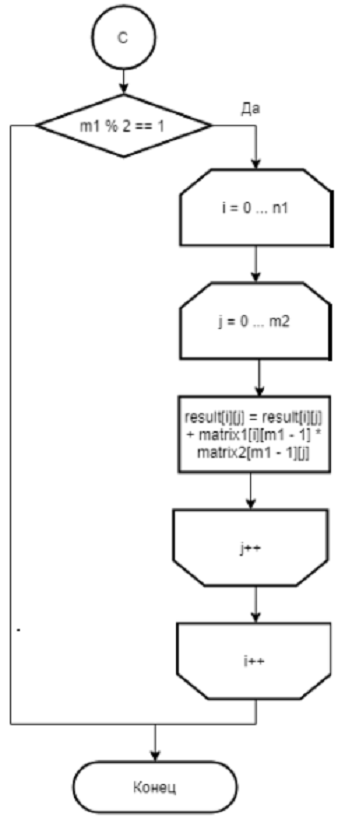
\includegraphics[width=0.6\linewidth]{inc/img/m_winograd2}}
	\caption{Схема алгоритма Винограда (продолжение)}
\end{figure}

\newpage
\section{Вывод}
В данном разделе были представлены требования к разрабатываемому ПО и разработаны схемы алгоритмов умножения матриц.